\documentclass[12pt]{article}
\usepackage[utf8]{inputenc}

\usepackage[margin=1in]{geometry}
\usepackage{color,soul}
\usepackage{xcolor}
\usepackage{array}
\usepackage{mhchem}
\usepackage{mathtools}

\DeclarePairedDelimiter\ceil{\lceil}{\rceil}
\DeclarePairedDelimiter\floor{\lfloor}{\rfloor}

\bibliographystyle{plos2015}


\begin{document}


\vspace*{0.2in}

% Title must be 250 characters or less.
\begin{flushleft}
{\Large
\textbf\newline{Adaptive dating and fast proposals: revisiting the phylogenetic relaxed clock model} % Please use "sentence case" for title and headings (capitalize only the first word in a title (or heading), the first word in a subtitle (or subheading), and any proper nouns).
}
\newline
% Insert author names, affiliations and corresponding author email (do not include titles, positions, or degrees).
\\
Jordan Douglas\textsuperscript{1,2*},
Rong Zhang\textsuperscript{1,2},
Remco Bouckaert\textsuperscript{1,2,3}
\\
\bigskip
\textbf{1} Centre for Computational Evolution,  University of Auckland, Auckland, New Zealand\\
\textbf{2} School of Computer Science, University of Auckland, Auckland, New Zealand\\
\textbf{3} Max Planck Institute for the Science of Human History, Jena, Germany\\
\bigskip


% Use the asterisk to denote corresponding authorship and provide email address in note below.
* jordan.douglas@auckland.ac.nz


\end{flushleft}


\section*{S2 Appendix: Well-calibrated simulation studies}


The methods presented and benchmarked in this paper were validated with well-calibrated simulation studies using the same model and operator scheme that was benchmarked. 
This was achieved using 100 simulated datasets (each with $N=30$ taxa and a $L=2000$ nt alignment).
The 95\% highest posterior density (HPD) intervals of each parameter during MCMC were calculated, and these intervals were compared with the `true' parameter values which the data was simulated under. 


The validation results are presented as plots (below). 
In each plot, blue and red vertical lines are 95\% HPD intervals, where blue intervals contain the true value and red intervals do not.
The number at the top of each plot is the coverage; that is the percentage of simulations where the `true' parameter value is within the 95\% HPD interval. 
If all parameters have coverage close to 95\%, then this suggests correctness of both methodology and implementation.

Overall, these experiments suggest that the operators presented in the main paper were correctly implemented.




\begin{figure}[!htb]
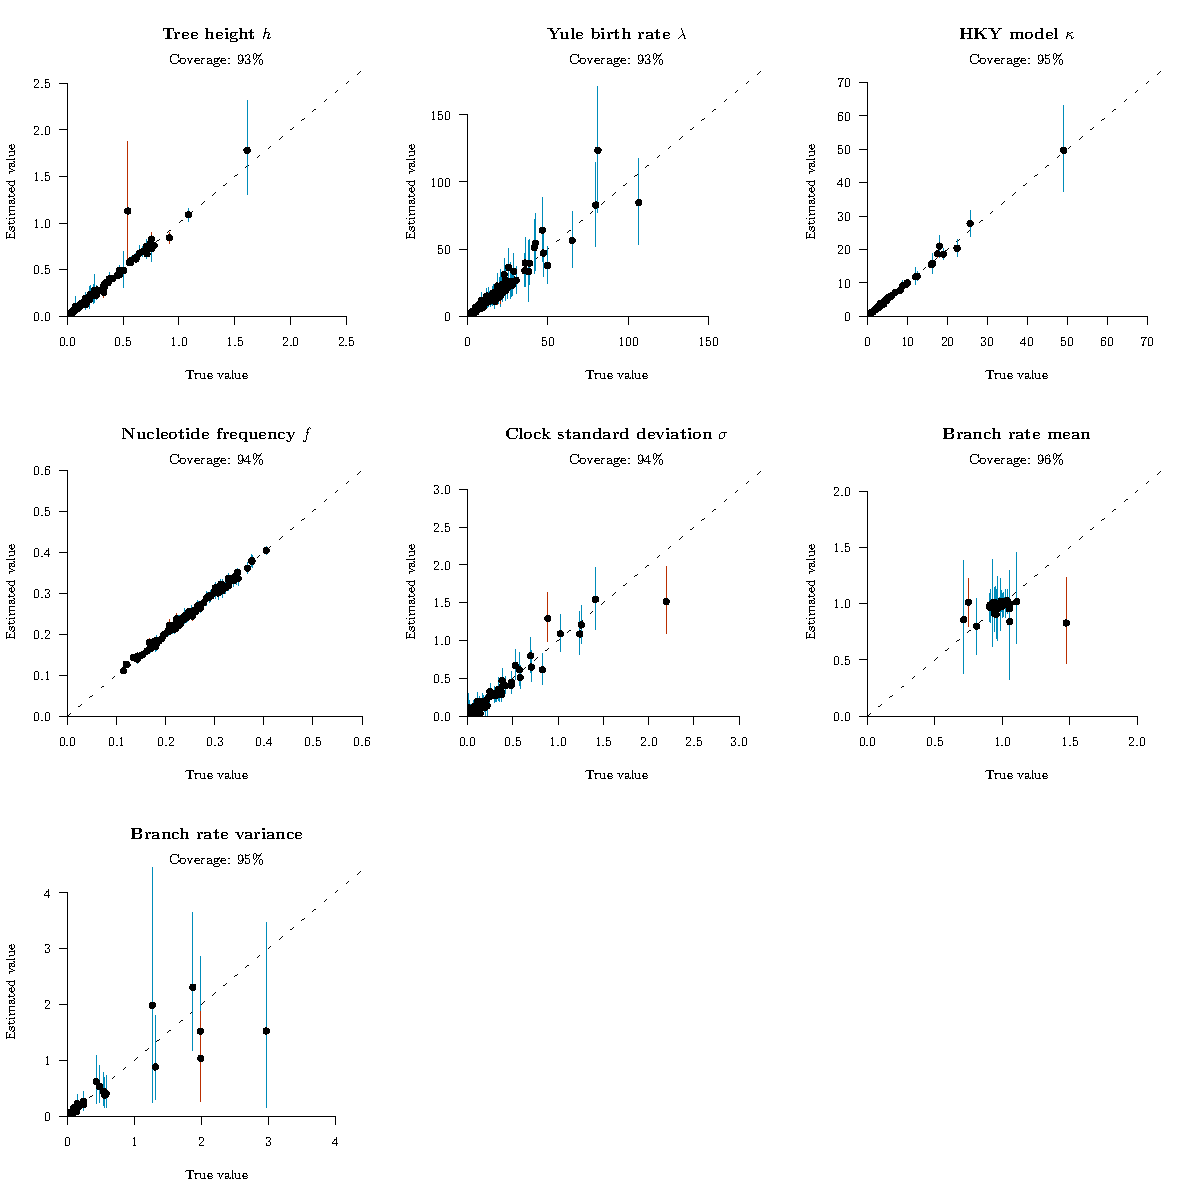
\includegraphics[width=\textwidth]{RatesWCSS/WCSS_cat_adaptive.pdf}
\caption{\textbf{The adapt (\textit{cat}) configuration.} }
\end{figure}


\begin{figure}[!htb]
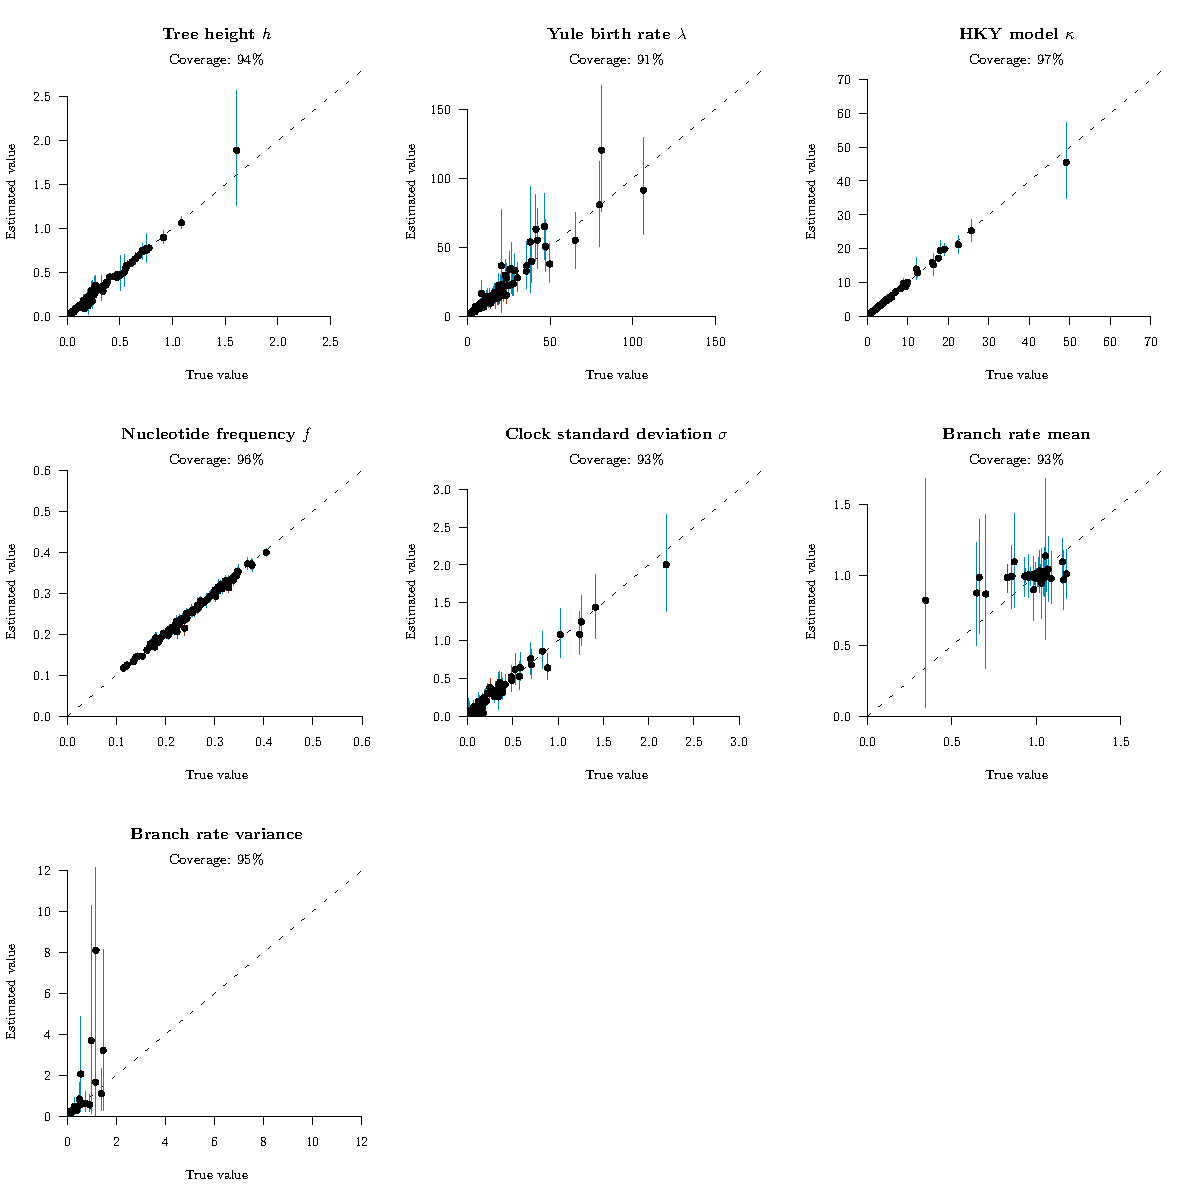
\includegraphics[width=\textwidth]{RatesWCSS/WCSS_real_adaptive.pdf}
\caption{\textbf{The adapt (\textit{real}) configuration.} }
\end{figure}


\begin{figure}[!htb]
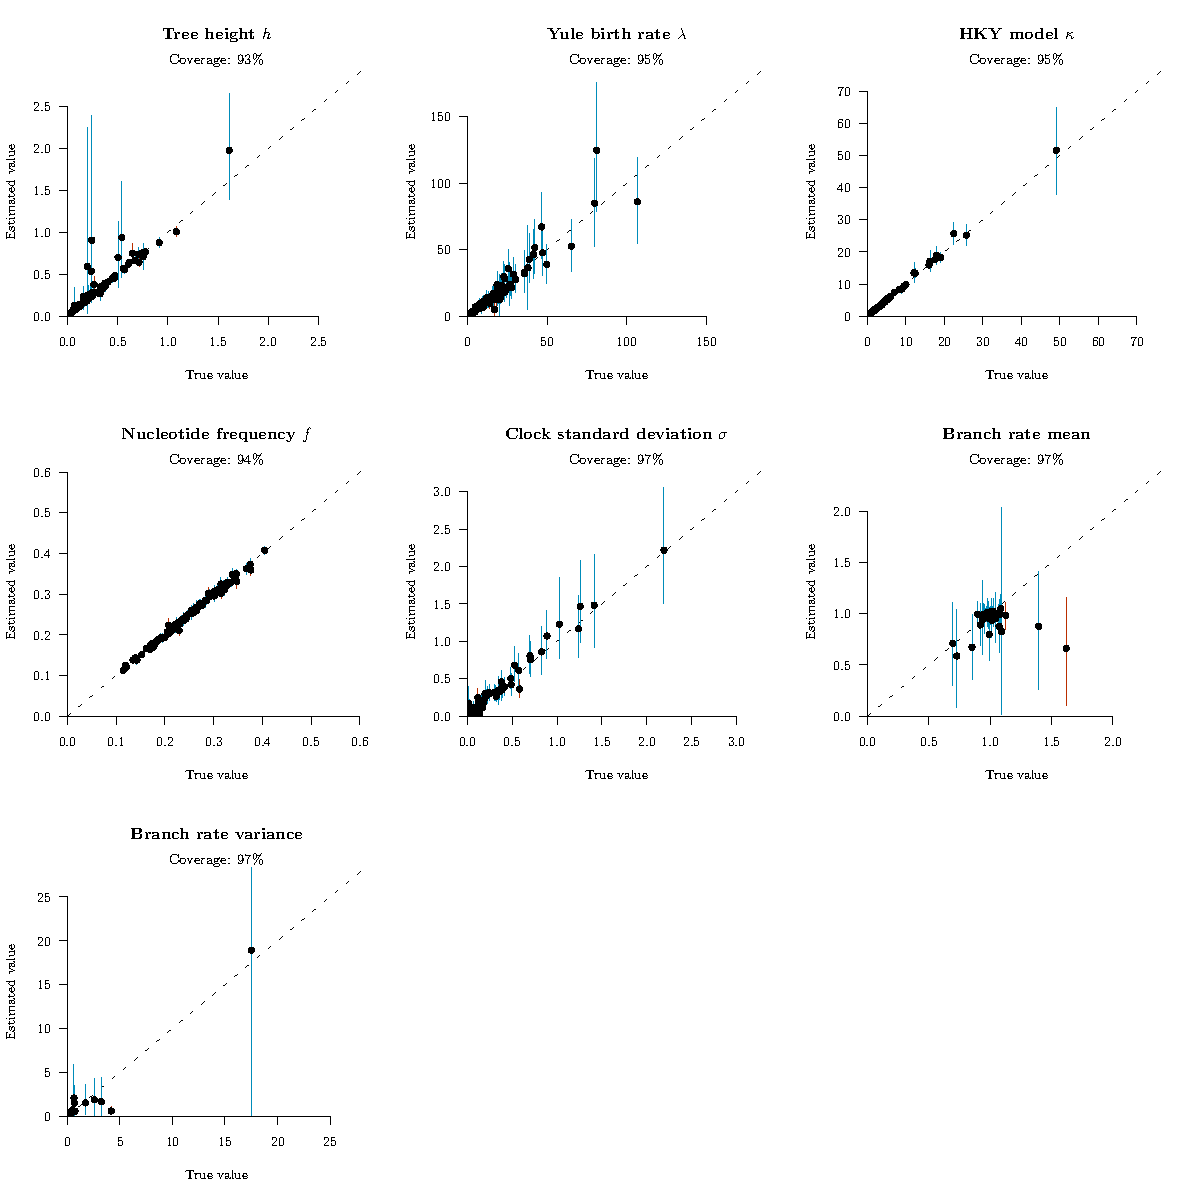
\includegraphics[width=\textwidth]{RatesWCSS/WCSS_quant_cached_adaptive.pdf}
\caption{\textbf{The adapt (\textit{quant}) configuration.} The constant distance operators were extended from \emph{real} to \emph{quant} as described in \textbf{S1 Appendix}.}
\end{figure}




\begin{figure}[!htb]
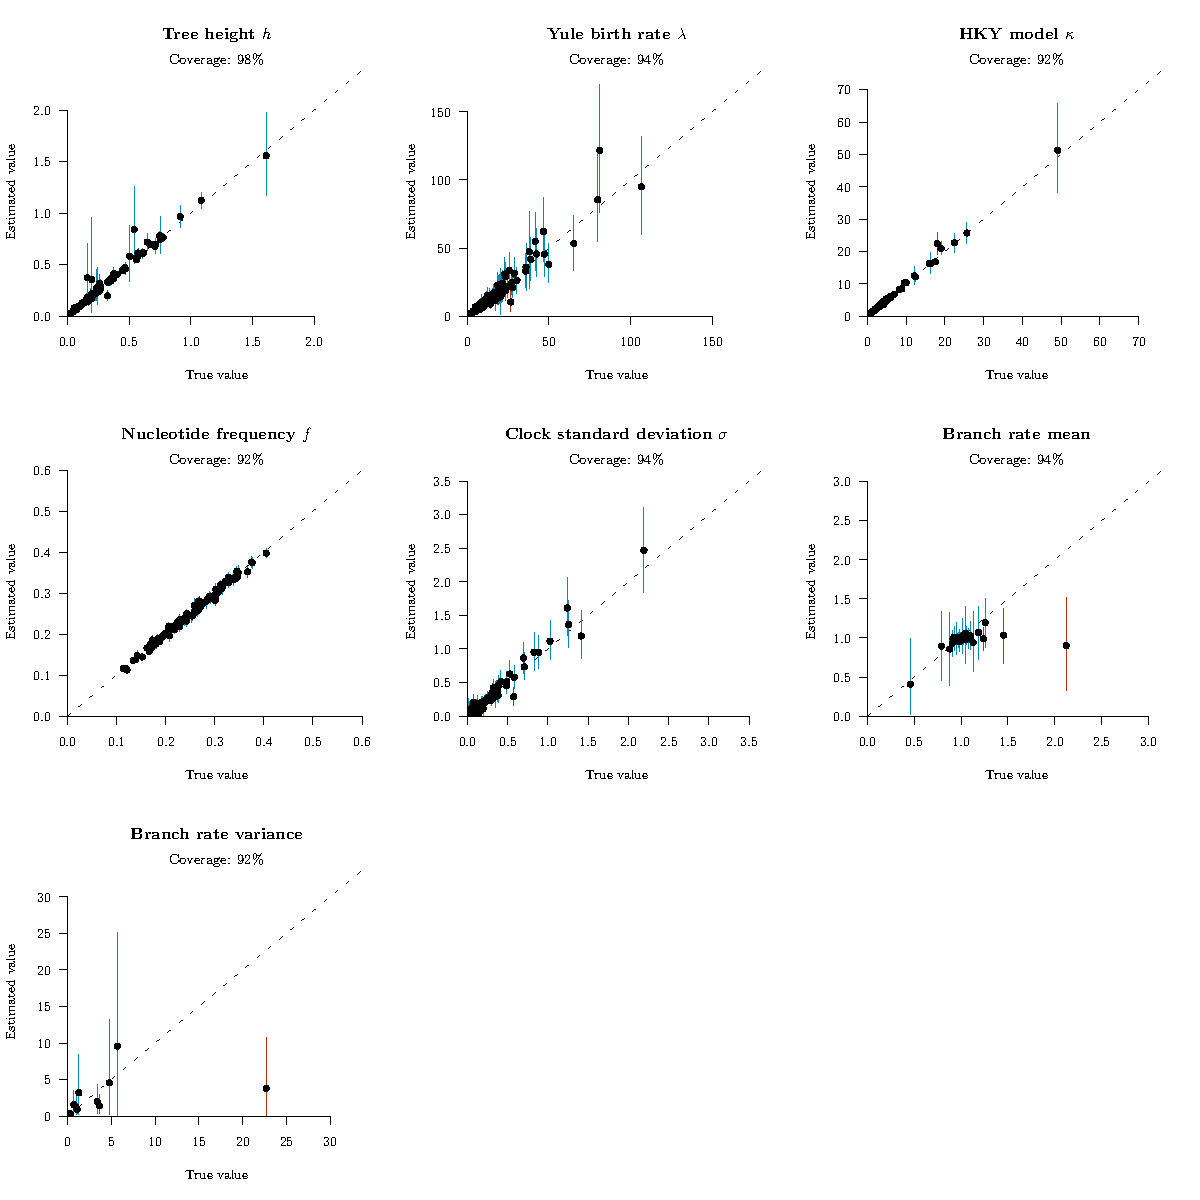
\includegraphics[width=\textwidth]{RatesWCSS/WCSS_AVMVN.pdf}
\caption{\textbf{The AVMVN configuration.} The adaptive NER operator, Bactrian proposals, and the \emph{real} configuration are also included.}
\end{figure}





%\bibliography{references}




\end{document}